
\documentclass[10pt,journal,onecolumn]{IEEEtran}
\usepackage[T1]{fontenc}
\usepackage[utf8]{inputenc}
\usepackage{cite}
\usepackage{url}
\usepackage{booktabs}
\usepackage{array}
\usepackage{longtable}
\usepackage{tabularx}
\usepackage{enumitem}
\usepackage{listings}
\usepackage{xcolor}
\usepackage{amsmath,amssymb}
\usepackage{tikz}
\usetikzlibrary{positioning,arrows.meta,shapes.geometric,fit}
\usepackage[hidelinks]{hyperref}
\lstset{basicstyle=\ttfamily\scriptsize,breaklines=true,columns=fullflexible,frame=single}
\setlist{nosep,leftmargin=*}
\title{JMCP V5 and JPCM-1.0: A Protocol-First Supervisory Control Plane for Autonomous Engineering, Tool Building, Voice Interaction, and Self-Improvement}
\author{Prepared for Jepson Taylor and NEVERHUMAN Systems\\June 2026}
\begin{document}
\maketitle
\begin{abstract}
Autonomous engineering systems increasingly combine language models, coding agents, browser agents, model-context tools, agent-to-agent protocols, CI systems, databases, memories, and user-facing assistants. The central risk is not lack of automation; it is lack of enforceable control, evidence, and attention management. This paper presents the final V5 design for the Joint Master Control Plane (JMCP) and its mandatory communication standard, Joint Process Control Messaging version 1.0.0 (JPCM-1.0). JMCP is defined as an assured supervisory control plane, not a chatbot, not an agent framework, not an MCP host, and not an observability dashboard. JPCM-1.0 defines the signed envelope, service cards, tool cards, data cards, model cards, capability leases, context contracts, work orders, tasks, evidence bundles, attention packets, approval packets, memory records, self-improvement proposals, tool-build proposals, and conformance reports required for every service that communicates with JMCP. The design emphasizes least authority, evidence-gated promotion, durable replay, voice-specific safety, user-attention minimization, live tool/data awareness, and governed self-improvement. The result is a blueprint for a software fab operating system: a control room for autonomous engineering that increases value while reducing user cognitive load.
\end{abstract}
\begin{IEEEkeywords}
AI agents, autonomous software engineering, control plane, protocol, observability, Model Context Protocol, Agent2Agent, capability security, evidence, provenance, voice interface, self-improvement, tool building.
\end{IEEEkeywords}

\section{Introduction}
Autonomous engineering is entering a regime in which the limiting factor is no longer whether an agent can write code, call tools, or search documentation. The limiting factor is whether a human can safely supervise many partially reliable actors that can touch repositories, build systems, databases, browsers, memories, and external services. A larger model does not solve the control problem. A better prompt does not solve the evidence problem. A dashboard does not solve the attention problem. A tool protocol does not solve the authority problem.

The Joint Master Control Plane (JMCP) is proposed as an assured supervisory control plane for this regime. The design goal is not to maximize visible automation, but to maximize useful, verified, low-noise progress under human intent. JMCP is the primary text and voice interface for the user, the authority kernel for machines, the evidence gate for promotion, the communication backbone for services, the task manager for all work, and the attention firewall that decides what must reach the user.

The companion protocol, Joint Process Control Messaging version 1.0.0 (JPCM-1.0), is the mandatory standard by which all services communicate with JMCP. This paper finalizes JPCM as a normative object model rather than a prose convention. Every service, tool, agent, datastore adapter, voice surface, and frontend module must either speak JPCM natively or run behind a constrained adapter. The schema delivered with this paper defines the envelope, actors, authority references, leases, work orders, tasks, evidence bundles, attention packets, approvals, service cards, tool cards, data cards, model cards, self-improvement proposals, tool-build proposals, and conformance reports.

\subsection{Thesis}
The correct abstraction for JMCP is not chatbot, agent framework, MCP host, A2A peer, CI wrapper, or observability dashboard. The correct abstraction is a software fab operating system: a supervisory control layer that monitors process health, allocates authority, routes work, detects faults, verifies outputs, preserves provenance, learns from experience, and exposes only the minimum useful information to the human.

\subsection{Contributions}
This paper contributes:
\begin{enumerate}
\item A destructive critique of the prior V4 corpus and a hardening response.
\item A final definition of what JMCP is and what it is not.
\item A protocol-first architecture in which JPCM-1.0 is mandatory for all services.
\item A complete task model including research, coding, deployment, memory, self-improvement, and automated tool building.
\item A user-attention model for bare-minimum escalation with drilldown.
\item A text and voice communication model with voice-specific safety controls.
\item A tool and data awareness model for live capability, risk, cost, and technology inventory.
\item An extreme future vector: JMCP as a self-hardening engineering foundry and trust fabric.
\end{enumerate}

\section{Hostile Review of the V5 Input Corpus}
The uploaded V5 corpus contains strong architecture candidates, protocol-first drafts, scorecards, and JSON envelope seeds. The strongest artifacts already recognize that JMCP must own authority and evidence. However, several failure modes remain.

\subsection{Protocol Is Still Too Easy To Treat As Ceremonial}
Several drafts define envelopes, but an envelope alone does not make a control plane. If payload semantics are not standardized, every adapter can smuggle authority through private fields. If tasks are not standardized, schedulers cannot compare work. If evidence is not standardized, promotion degenerates into trust in self-reported logs. V5 addresses this by defining the JPCM-1.0 schema as the normative object model.

\subsection{Authority Must Be Checked At The Effect Boundary}
A lease is meaningless unless the service that performs the side effect checks it. If JMCP grants a lease but a downstream adapter ignores it, the system is a dashboard. V5 requires lease-aware conformance levels and forbids production effects through services below C3, with R4/R5 actions requiring replay-safe C4 or full C5 conformance.

\subsection{Evidence Can Be Forged Or Misleading}
Logs, CI, tests, and agent summaries can all be produced by the same compromised actor. Evidence must carry provenance, signature, trust class, reproducibility, and independence. V5 introduces evidence quality tiers from E0 claims to E5 formal or human-approved proof.

\subsection{Voice Is A Separate Security Boundary}
Voice adds speaker ambiguity, transcription errors, replay attacks, urgency bias, and social-engineering risk. Treating voice as merely another text input is unsafe. V5 requires original audio or approved redacted audio, transcript, redacted transcript, speaker confidence, intent confidence, and risk-based confirmation policy.

\subsection{Self-Improvement Can Corrupt The Governor}
A self-improving control plane can weaken its own controls, poison memory, change policy thresholds, or overfit to local success. V5 makes self-improvement a first-class task type with hypothesis, experiment, shadow mode, evaluation, promotion gates, and rollback.

\subsection{Automated Tool Building Creates Supply-Chain Debt}
A system that can build tools can also create unmaintained, insecure, or overlapping infrastructure. V5 requires build-vs-buy analysis, ownership, threat modeling, security plan, evaluation plan, conformance level, promotion plan, and retirement plan.

\section{Definition: What JMCP Is}
JMCP is an assured supervisory control plane for autonomous engineering and knowledge work. It is the primary user interface, authority plane, communication backbone, workflow kernel, evidence gate, attention broker, tool and data awareness layer, cognition governor, memory governor, standards compiler, and self-improvement governor.

JMCP owns the following decisions: whether a task exists, which actor may perform it, what context may be used, what tools may be invoked, what data may be read or written, what side effects are allowed, what evidence is required, what gets promoted, what memory is retained, and what the user must see.

\section{Negative Definition: What JMCP Is Not}
JMCP is not a chatbot. Chat is a surface. JMCP is not an agent framework. Agents are replaceable workers. JMCP is not an MCP host. MCP standardizes access to tools and context, but it does not by itself provide enterprise authority, evidence promotion, or user-attention governance. JMCP is not an A2A participant in the peer sense. A2A agents may coordinate, but JMCP is the controller. JMCP is not a CI wrapper. CI is evidence input, not a proof root. JMCP is not a memory bucket. Memory is governed, evidenced, scoped, expiring, and revocable.

\section{Related Work and Gap}
MCP provides a standard way for model applications to reach tools and context, including utilities such as progress, cancellation, error reporting, and logging. It also explicitly acknowledges security and trust concerns because tool and data access can lead to arbitrary code execution paths. A2A focuses on communication and collaboration among opaque agentic applications. OpenTelemetry provides semantic conventions for generative AI telemetry. CloudEvents standardizes common event metadata. NATS JetStream provides durable persistence and replay. OWASP catalogs LLM-specific risks including prompt injection, insecure outputs, model denial of service, supply-chain vulnerabilities, sensitive information disclosure, insecure plugin design, excessive agency, and overreliance.

These systems are necessary but insufficient. The missing system is a common authority and evidence plane that controls agents, tools, tasks, data, memory, and user attention together. JMCP fills that gap by making protocol conformance, leases, context contracts, evidence bundles, and attention packets mandatory.

\section{Reference Architecture}
Figure~\ref{fig:arch} shows the core architecture. The user communicates by text, voice, and cockpit UI. JMCP Core owns authority, scheduling, attention, memory governance, and evidence. External services communicate only through JPCM or adapters.

\begin{figure}[!t]
\centering
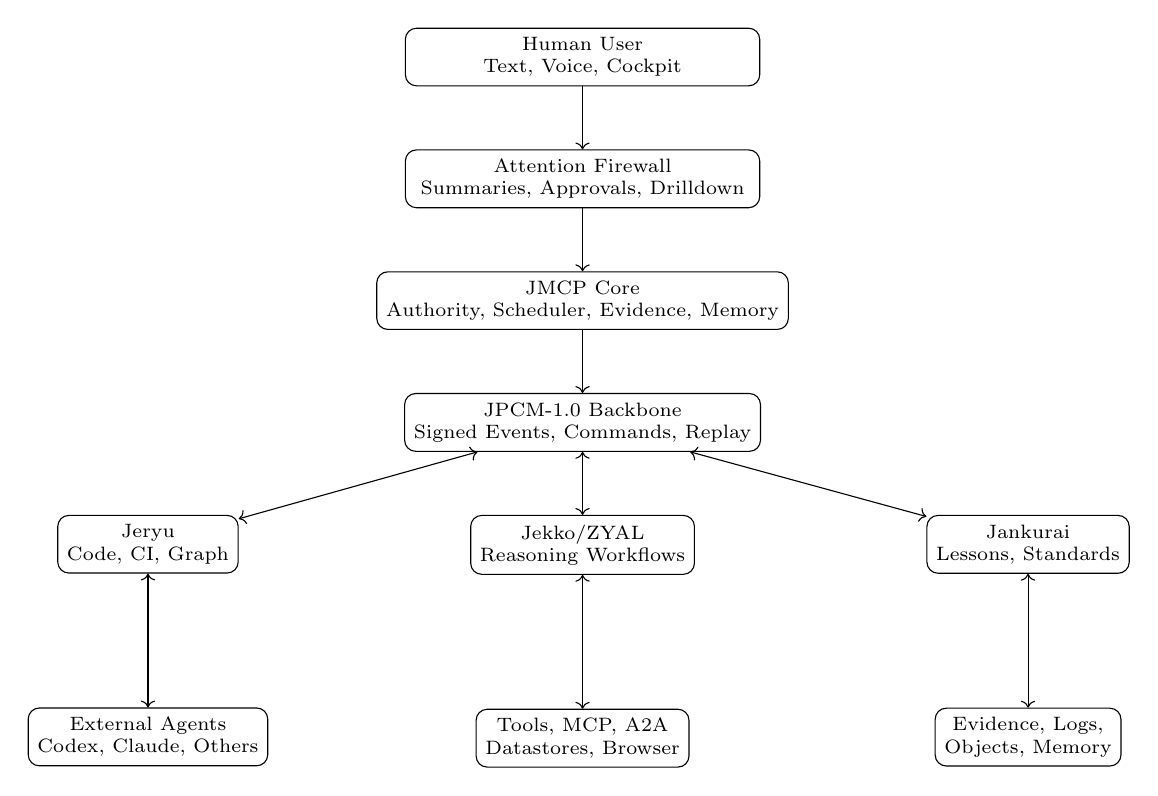
\begin{tikzpicture}[node distance=0.8cm, every node/.style={font=\scriptsize}, box/.style={draw, rounded corners, align=center, minimum width=2.2cm, minimum height=0.7cm}, wide/.style={draw, rounded corners, align=center, minimum width=4.5cm, minimum height=0.7cm}]
\node[wide] (user) {Human User\\Text, Voice, Cockpit};
\node[wide, below=of user] (attn) {Attention Firewall\\Summaries, Approvals, Drilldown};
\node[wide, below=of attn] (core) {JMCP Core\\Authority, Scheduler, Evidence, Memory};
\node[wide, below=of core] (jpcm) {JPCM-1.0 Backbone\\Signed Events, Commands, Replay};
\node[box, below left=0.8cm and 2.1cm of jpcm] (jeryu) {Jeryu\\Code, CI, Graph};
\node[box, below=0.8cm of jpcm] (jekko) {Jekko/ZYAL\\Reasoning Workflows};
\node[box, below right=0.8cm and 2.1cm of jpcm] (jank) {Jankurai\\Lessons, Standards};
\node[box, below=1.7cm of jeryu] (agents) {External Agents\\Codex, Claude, Others};
\node[box, below=1.7cm of jekko] (tools) {Tools, MCP, A2A\\Datastores, Browser};
\node[box, below=1.7cm of jank] (stores) {Evidence, Logs,\\Objects, Memory};
\draw[->] (user) -- (attn);
\draw[->] (attn) -- (core);
\draw[->] (core) -- (jpcm);
\draw[<->] (jpcm) -- (jeryu);
\draw[<->] (jpcm) -- (jekko);
\draw[<->] (jpcm) -- (jank);
\draw[<->] (jeryu) -- (agents);
\draw[<->] (jekko) -- (tools);
\draw[<->] (jank) -- (stores);
\end{tikzpicture}
\caption{JMCP V5 reference architecture. JMCP owns authority and attention; all services communicate through JPCM-1.0 or constrained adapters.}
\label{fig:arch}
\end{figure}

\section{JPCM-1.0 Protocol}
JPCM-1.0 is the mandatory communication standard. It is not optional telemetry. It is the control fabric. A service cannot participate in authority-bearing work unless it validates and emits JPCM messages.

\subsection{Envelope}
Every message includes version, id, family, type, source, subject, timestamp, tenant, cell, trace id, correlation id, actor, authority, risk, data class, delivery, schema reference, payload hash, signature, and payload. The delivered JSON Schema is normative.

\subsection{Message Families}
The required message families are intent, command, event, observation, task, lease, evidence, attention, approval, memory, service, tool, data, model, voice, policy, protocol, conformance, audit, and error. Each family maps to payload objects in the schema.

\subsection{Delivery Classes}
JPCM defines telemetry-at-most-once, event-at-least-once, command-exactly-once-effect, audit-append-only, ui-low-latency, and voice-low-latency. Exactly-once effect is implemented through idempotency keys and an effect ledger, not by assuming perfect transport.

\subsection{Conformance Levels}
C0 systems are wrapped legacy systems. C1 systems emit valid envelopes. C2 systems are lease-aware. C3 systems emit evidence. C4 systems are replay-safe. C5 systems are full control participants. Production side effects require at least C3, and high-risk actions require C4 or C5.

\section{Communication Backbone}
The recommended backbone uses NATS JetStream for durable streams and replay, PostgreSQL for materialized state, an object or content-addressed store for evidence, a graph store for causal and code relationships, vector/search projections for governed retrieval, OpenTelemetry for traces and metrics, WebSocket/SSE for cockpit streams, and WebRTC or equivalent media transport for voice.

The backbone must survive duplicate messages, out-of-order events, partial partitions, producer crashes, consumer crashes, stale schemas, poisoned adapters, and replay. Therefore, every side-effecting command must use an idempotency key; every materializer must be rebuildable; every audit event must be append-only; and every adapter must fail closed when authority fields are invalid.

\section{Task And Workflow Management}
A work order captures user or policy intent. A task is the schedulable unit of work. Tasks form DAGs with dependencies, budgets, risk, required leases, required evidence, and state history. The task state machine is shown in Figure~\ref{fig:task}.

\begin{figure}[!t]
\centering
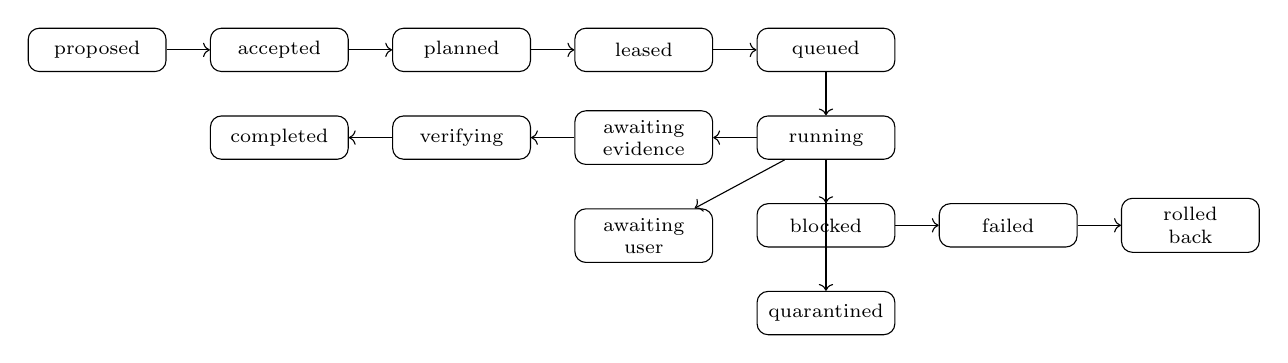
\begin{tikzpicture}[node distance=0.55cm, every node/.style={font=\scriptsize}, s/.style={draw, rounded corners, align=center, minimum width=1.75cm, minimum height=0.55cm}]
\node[s] (p) {proposed};
\node[s, right=of p] (a) {accepted};
\node[s, right=of a] (pl) {planned};
\node[s, right=of pl] (l) {leased};
\node[s, right=of l] (q) {queued};
\node[s, below=of q] (r) {running};
\node[s, left=of r] (e) {awaiting\\evidence};
\node[s, left=of e] (v) {verifying};
\node[s, left=of v] (c) {completed};
\node[s, below=of e] (u) {awaiting\\user};
\node[s, below=of r] (b) {blocked};
\node[s, right=of b] (f) {failed};
\node[s, right=of f] (rb) {rolled\\back};
\node[s, below=of b] (x) {quarantined};
\draw[->] (p)--(a); \draw[->] (a)--(pl); \draw[->] (pl)--(l); \draw[->] (l)--(q); \draw[->] (q)--(r);
\draw[->] (r)--(e); \draw[->] (e)--(v); \draw[->] (v)--(c);
\draw[->] (r)--(u); \draw[->] (r)--(b); \draw[->] (b)--(f); \draw[->] (f)--(rb); \draw[->] (r)--(x);
\end{tikzpicture}
\caption{JPCM task state machine. Risky transitions require leases, evidence, and sometimes user approval.}
\label{fig:task}
\end{figure}

JPCM-1.0 explicitly supports research, knowledge compression, architecture, code change, repo creation, refactoring, bug hunting, security scanning, dependency updates, test generation, CI, release, deployment, rollback, incident diagnosis, data query, data migration, memory proposal, lesson publication, policy change, protocol change, adapter registration, service onboarding, tool evaluation, tool building, tool retirement, self-improvement, model routing, agent delegation, browser work, voice interaction, approval, cost optimization, observability rules, conformance testing, and red-team tasks.

\section{Authority, Leases, And Context Contracts}
Capability leases are scoped, expiring, revocable grants. They bind actor, capability, target, task, work order, risk ceiling, context, cost, runtime, network policy, file roots, required evidence, and revocation subject. Context contracts define allowed sources, forbidden sources, redaction, memory policy, and expiration. A command without both a valid lease and a compatible context contract fails closed.

\section{Evidence Architecture}
An evidence bundle contains evidence items, provenance, quality tier, verdict, reviewer, and gaps. Evidence items include claims, transcripts, logs, traces, metrics, test results, CI runs, static analysis, dynamic analysis, security scans, SBOMs, provenance, signatures, screenshots, diffs, patches, reproducibility scripts, human reviews, policy decisions, red-team results, cost reports, benchmarks, and runtime observations.

\begin{table}[!t]
\centering
\caption{Evidence tiers}
\begin{tabular}{lll}
\toprule
Tier & Meaning & Allowed use\\
\midrule
E0 & Claim & Diagnosis only\\
E1 & Log/transcript & Weak support\\
E2 & Test/local check & Low-risk changes\\
E3 & Independent check & Repository changes\\
E4 & Reproducible attestation & Release/prod/security\\
E5 & Formal or human-approved & Irreversible/policy/protocol\\
\bottomrule
\end{tabular}
\end{table}

\section{The Attention Firewall}
JMCP protects the user from noise by default. It converts raw activity into attention packets. An attention packet has level, summary, decision-needed flag, options, risks, drilldown references, modality, and expiration. The default is silence for safe work, digest for completed progress, heads-up for meaningful change, decision for material choices, urgent for incidents.

The attention firewall is not a hiding mechanism. It is a compression and escalation mechanism. Every packet must support drilldown into work order, tasks, evidence, logs, traces, and source artifacts.

\section{Text And Voice Interface}
The text interface accepts goals, constraints, approvals, corrections, and drilldown requests. The voice interface accepts conversational commands and status queries. Voice messages are first-class JPCM events with audio artifact, transcript, redacted transcript, language, ASR model, speaker confidence, intent confidence, and confirmation policy. Voice commands that create external, production, expensive, credential, legal, or irreversible effects require confirmation unless a user-approved standing policy says otherwise.

\section{Tool And Data Awareness}
JMCP must be 100 percent tool and data aware in the operational sense: it knows what tools exist, what actions they expose, what data they touch, what side effects they create, what schemas they use, what they cost, what their conformance level is, what evidence qualifies them, what failures they have exhibited, and whether they should be adopted, trialed, assessed, held, built, wrapped, or retired.

Service cards, tool cards, data cards, and model cards are mandatory. The technology radar classifies capabilities into Adopt, Trial, Assess, and Hold. Missing capability detection can create tool-build proposals, but tool building is governed work, not free-form automation.

\section{Self-Improvement}
Self-improvement is a task class, not a permission. JMCP may improve prompts, policies, schedulers, model routing, memory indexes, evidence graders, user-attention thresholds, adapters, tools, and observability rules. It may not silently weaken authority, evidence, audit, privacy, or user-attention controls.

Every self-improvement proposal requires a hypothesis, target component, expected gain, risk, experiment plan, promotion gates, rollback plan, shadow-mode requirement, and approval rule. Promotion requires comparison against baseline and monitoring after canary.

\section{Automated Tool Building}
Automated tool building is allowed because JMCP must become more powerful over time. It is dangerous because it creates supply-chain and maintenance risk. A tool-build proposal must define the problem, build-vs-buy decision, alternatives considered, API, inputs, outputs, side effects, owner, risk, security plan, evaluation plan, promotion plan, and retirement plan. Tools built by agents start in an isolated cell and cannot perform production side effects until conformance and independent verification pass.

\section{Security Model}
JMCP assumes compromised agents, hallucinated plans, prompt injection, tool poisoning, memory poisoning, forged evidence, false-green CI, supply-chain compromise, sandbox escape, adapter trust laundering, credential leakage, model denial of service, voice replay, partial network failure, stale schemas, and user overload.

Controls include signed JPCM envelopes, workload identity, leases, context contracts, deny-by-default networking, brokered secrets, sandboxing, policy-as-code, SBOMs, provenance, signed releases, conformance tests, immutable evidence, independent verification, attention thresholds, voice confirmations, and quarantine.

\section{User-Minimal Communication Policy}
JMCP decides what information to share through a policy function over risk, uncertainty, reversibility, cost, user preference, task criticality, novelty, and time sensitivity. The function should minimize user attention cost subject to preserving informed consent for material decisions. Raw logs should not reach the user unless requested. The user should see decisions, not machinery.

\section{Frontend}
The frontend is a high-performance React/Vite cockpit. It shows attention inbox, command/voice rail, work graph, system map, evidence drilldown, risk cockpit, tool/data radar, memory browser, and incident timeline. It uses virtualized views, materialized summaries, WebSocket/SSE streams, and local graph rendering. It is not the source of authority; it is a user and operator surface over JPCM state.



\section{Risk, Autonomy, And Attention Tiers}
JMCP treats risk, autonomy, and attention as separate axes. Risk describes the worst plausible consequence of an action. Autonomy describes what the system may do without the user. Attention describes what the user should see. Conflating these axes is dangerous: a low-risk task may still require attention if it changes product direction, and a high-risk observation may require no authority if it is read-only.

\subsection{Risk Tiers}
R0 is observe-only. R1 is local safe work with no material side effect. R2 is reversible work such as branch-local code changes. R3 touches sensitive data, cross-repo behavior, security posture, or user-visible artifacts. R4 touches production, money, credentials, external systems, or expensive compute. R5 is irreversible, legally significant, destructive, public, or security-critical. Each tier maps to minimum evidence and approval rules.

\subsection{Autonomy Tiers}
A0 is suggest-only. A1 may prepare artifacts but not change durable state. A2 may execute reversible sandboxed work. A3 may create branches, tests, and pull requests under policy. A4 may promote low-risk changes when evidence is sufficient. A5 may handle pre-authorized production workflows but only within explicit standing policy and audit. The default for new services is A0 until conformance and qualification improve.

\subsection{Attention Tiers}
Silent means no user notification. Digest means summarized later. Heads-up means visible but non-blocking. Decision means the user must choose among options. Urgent means immediate interruption. Incident means the system should provide a concise situation report, blast radius, current containment, and safe choices.

\section{JPCM Field Semantics}
The JPCM envelope is intentionally redundant. Distributed systems fail at boundaries, so authority, risk, delivery, and trace fields must travel with each message rather than being inferred from ambient connection state.

\begin{longtable}{p{0.20\linewidth}p{0.28\linewidth}p{0.42\linewidth}}
\caption{JPCM mandatory envelope fields}\label{tab:envelope}\\
\toprule
Field & Purpose & Failure prevented\\
\midrule
\endfirsthead
\toprule
Field & Purpose & Failure prevented\\
\midrule
\endhead
jpcm\_version & Protocol compatibility & Silent schema drift\\
message\_id & Global identity & Duplicate processing\\
message\_family & Routing class & Private side-channel semantics\\
message\_type & Domain operation & Ambiguous adapter behavior\\
source & Producer identity & Attribution loss\\
subject & Backbone routing & Unstructured event streams\\
issued\_at & Time semantics & Replay ambiguity\\
tenant, cell & Boundary & Cross-tenant leakage\\
trace\_id & Distributed trace & Undebuggable workflows\\
correlation\_id & Request relation & Lost causality\\
actor & Actual actor & Trust laundering\\
authority & Decision reference & Ambient permission\\
risk & Consequence model & Silent escalation\\
data\_class & Information sensitivity & Data leakage\\
delivery & Reliability contract & Replay side effects\\
schema\_ref & Payload contract & Parser drift\\
payload\_hash & Integrity & Payload substitution\\
signature & Authenticity & Forged commands\\
payload & Object body & Underspecified action\\
\bottomrule
\end{longtable}

\section{Protocol Subjects And Routing Discipline}
The subject namespace is deliberately human-readable and machine-checkable. It begins with \texttt{jpcm} and includes family, target, and domain-specific identifiers. A service must subscribe only to subjects that correspond to declared capabilities in its service card. Wildcard subscriptions are allowed for observability and audit services, but not for side-effecting workers unless the lease explicitly allows it.

Subject authorization is evaluated before payload parsing. This prevents a malicious actor from sending a plausible payload to a forbidden operational lane. Subject policy also makes backpressure targeted: a noisy telemetry stream should not block approval, lease revocation, or incident messages.

\section{Service Registration And Qualification}
Service registration is a protocol event, not a configuration file hidden in deployment. A service registers a service card, proves workload identity, declares schemas, declares side effects, declares data access, and provides qualification evidence. JMCP then assigns a conformance level. A service may be healthy but unqualified; health means it is alive, not that it is trusted.

Registration is renewed periodically. Expired qualification downgrades service autonomy. A service that changes version, endpoint, sandbox, dependency base, schema, or side-effect declaration must re-register. JMCP should compare new service cards against previous cards and emit attention packets for material changes.

\section{Adapter Semantics}
Adapters are necessary because the ecosystem includes MCP servers, A2A agents, CLIs, browser tools, CI systems, SQL and NoSQL databases, repository APIs, and model providers. However, adapters are also one of the highest-risk surfaces because they can translate away authority semantics. V5 therefore uses the following adapter rules.

First, an adapter must preserve actor chain. If a Codex-like agent calls an MCP tool through an adapter, the resulting command must name the original agent, the adapter, the lease, and the task. Second, an adapter must fail closed on unsupported semantics. If MCP or A2A lacks a field equivalent to a JPCM lease or evidence requirement, the adapter must not invent a permissive default. Third, the adapter must record translation evidence: input message, normalized command, rejected fields, and policy decision. Fourth, adapters are scoped to cells. A browser adapter in a research cell cannot mutate a production datastore.

\section{Integration With Jeryu, Jankurai, And Jekko/ZYAL}
Jeryu is the code, CI, git, and graph reality plane. JMCP uses it to answer what code exists, how files relate, which tests cover which paths, what CI says, and what would be affected by a change. Jeryu evidence is strong when it is independently produced and signed; it is weaker when generated by the same actor that proposed the code.

Jankurai is the lessons, standards, audit, and global-tool lane. JMCP uses Jankurai to push evidence-backed lessons learned from incidents, bugs, false positives, bad agent behavior, coding standards, and cross-repo tools. A local lesson cannot become global until it has scope, provenance, confidence, expiry, and contradiction policy.

Jekko/ZYAL is the cognition and workflow programming layer. JMCP uses it for smarter decomposition, reasoning workflows, memory operations, and agent scripts. Jekko/ZYAL does not own authority. It can propose and execute under lease, but JMCP decides whether the work is allowed and whether the output is promoted.

\section{Memory Governance}
Memory is one of the most dangerous capabilities in an autonomous system because it converts past observations into future bias. JMCP distinguishes temporary context, task memory, repo knowledge, process metrics, lessons, preferences, anti-patterns, and global standards. Each memory record has scope, provenance, confidence, TTL, promotion state, and contradiction references.

Memory write is a proposal, not a fact. The memory governor checks whether the proposed memory is supported by evidence, whether it contradicts existing memory, whether it is too broad, whether it contains sensitive data, and whether it needs expiration. Memory promotion can require human approval when the memory changes policy, coding standards, global agent behavior, or user preferences.

\section{Evidence Anti-Theater Controls}
Evidence theater occurs when a system produces artifacts that look rigorous but do not actually reduce uncertainty. JMCP counters this through independence, reproducibility, diversity, and adversarial checks. A high-risk code change should not be promoted solely because the same agent wrote tests and passed them. A release should not be promoted solely because CI is green if the CI definition changed in the same pull request. A security fix should not be promoted solely because static analysis stopped warning if the warning was suppressed.

JPCM evidence bundles therefore include producer identity, trust level, artifact digest, collection time, and summary. Promotion policy can require evidence from multiple producers, such as Jeryu graph impact, deterministic tests, static analysis, independent review, and runtime simulation.

\section{Scheduling And Bottleneck Control}
JMCP scheduling is not a FIFO queue. It is a value, risk, deadline, dependency, and learning optimizer. It should always have useful background work, but background work must not starve user-directed work or incident response. Scheduling inputs include priority, risk reduction, unblock value, expected user value, learning value, estimated cost, uncertainty, deadline, affected repositories, required specialists, and current system load.

The scheduler should detect bottlenecks such as overloaded CI, flapping tests, slow review loops, missing tools, high agent retry rates, repeated memory contradictions, expensive model routes, and high user-interruption rates. Bottleneck diagnosis can create work orders: improve test isolation, build a missing graph query, retire a noisy tool, or add a conformance check.

\section{Data Model And Materialized Views}
The JPCM event stream is the source of audit truth, but user interfaces and schedulers need materialized views. Recommended relational tables include work\_orders, tasks, task\_dependencies, leases, approvals, evidence\_bundles, evidence\_items, attention\_packets, service\_cards, tool\_cards, data\_cards, model\_cards, memory\_records, conformance\_reports, and effect\_ledger. Graph projections connect repos, files, owners, tests, tasks, agents, tools, evidence, and incidents. Vector/search projections index governed memory and document evidence, never raw secrets.

Materializers must be replayable from the event stream. Rebuilding a projection must not re-execute side effects. This is why the effect ledger is separate from materialized state.

\section{Policy Model}
Policy decides whether a command may proceed. Policy inputs include actor, service conformance, task state, lease, context contract, risk tier, autonomy tier, data class, target, time, cost, evidence requirements, user standing policy, and incident mode. Policy outputs include allow, deny, require approval, require more evidence, require lower-risk plan, quarantine, or escalate.

Policy must be tested like code. Every policy change is a protocol or policy task with before/after examples, red-team cases, migration plan, and rollback. A self-improvement process may propose policy changes but may not promote them without gatekeeping.

\section{Voice Command Threat Model}
Voice failures include wrong speaker, wrong transcript, wrong intent, background speech, replayed command, synthesized voice, rushed confirmation, secret readout, and unsafe low-friction approval. JMCP treats every voice command as an evidence-producing session. The system should prefer short verbal acknowledgments and move complex detail to the visual cockpit. For example, a voice request to deploy should produce a spoken summary such as: ``I need confirmation because this touches production. I sent the evidence packet to the cockpit.''

\section{Frontend Drilldown Model}
The cockpit should avoid showing the user an event firehose. The default screen is an attention inbox and current work summary. Drilldown proceeds from attention packet to work order, from work order to task DAG, from task to actor and lease, from actor to service/tool/model card, from task to evidence bundle, from evidence to artifacts, and from artifacts to raw logs, traces, diffs, or audio transcripts. Every drilldown preserves causality and risk context.

\section{Automated Tool-Building Governance}
Tool-building starts with a capability gap. The system must ask whether an existing tool can solve the problem, whether wrapping is safer than building, whether the tool will be reused, who owns it, what side effects it has, what data it needs, how it will be tested, how it will be sandboxed, how it will be promoted, and how it will be retired. Tools that lack owners or retirement plans should not be promoted beyond experimentation.

A generated tool should begin with no network and no credentials. It should produce a service card and tool card. It should pass unit tests, integration tests, security checks, dependency scans, conformance tests, and fault injection. Only after shadow use and evidence review may it receive broader leases.

\section{Self-Improvement Governance}
A self-improvement proposal is judged by whether it improves measurable outcomes without weakening controls. Examples of acceptable metrics include lower user interruption rate at equal or better safety, lower cost per completed work order, higher conformance pass rate, faster incident diagnosis, fewer false-positive memory recalls, better task decomposition, and better evidence sufficiency. Examples of unacceptable metrics include more tasks completed by ignoring evidence, lower latency by skipping policy, or higher agent autonomy by hiding risk.

Self-improvement uses shadow mode whenever possible. In shadow mode, the new policy, router, memory index, or scheduler makes predictions without controlling real actions. JMCP compares shadow decisions to production decisions, evaluates differences, and promotes only when the improvement clears gates.

\section{Disaster Recovery And Replay}
Disaster recovery begins with durable JPCM audit streams and immutable evidence artifacts. The system must be able to rebuild materialized state from events, but commands must not reapply side effects. The effect ledger stores idempotency keys, target, requested effect, result, and evidence reference. During replay, materializers reconstruct state and skip effect execution.

Recovery tests must simulate broker restart, service crash, duplicate command, lost consumer offset, schema upgrade, adapter quarantine, and partial evidence-store outage. A control plane that cannot recover without duplicating side effects is not safe enough for autonomous work.

\section{Conformance Test Suite}
The conformance suite validates schema, signatures, subject policy, lease rejection, lease expiry, context contract rejection, evidence bundle creation, attention packet creation, idempotency, replay safety, backpressure handling, error message structure, service card renewal, tool card side-effect declaration, data card classification, model card disallowed-use enforcement, voice confirmation, self-improvement shadow mode, and tool-build promotion. Passing conformance is evidence; it is not permanent trust. Conformance expires.

\section{Reference Deployment Topology}
A minimal local deployment can run JPCM gateway, authorityd, schedulerd, evidenced, attentiond, registryd, PostgreSQL, object store, and cockpit. A production deployment should separate cells by network policy, run adapters in constrained sandboxes, isolate secrets, replicate event streams, use signed builds, collect OpenTelemetry, and run conformance and red-team tests in CI. High-risk cells should have separate credentials, separate network egress, and explicit approval policies.

\section{Economic And Performance Model}
JMCP should optimize for value per user attention minute, not only tasks per hour. Useful economic metrics include cost per verified task, cost per evidence bundle, model spend per successful work order, CI minutes per merged change, human approvals per week, avoided incidents, avoided duplicate work, and time saved through automatic drilldown. Performance metrics include p95 message validation latency, scheduler decision latency, task materialization latency, cockpit update latency, voice partial transcript latency, and replay recovery time.


\section{Implementation Plan}
Phase 0 builds schemas and conformance tests. Phase 1 builds JPCM gateway, authorityd, service registry, and task materializer. Phase 2 integrates Jeryu, Jankurai, Jekko/ZYAL, GitHub, CI, SQL, and basic frontend. Phase 3 adds evidence store, attention firewall, voice, and model/agent adapters. Phase 4 adds self-improvement and tool-building cells. Phase 5 adds predictive process control, cross-repo optimization, and autonomous R\&D workflows.

\section{Evaluation}
Evaluation must measure conformance pass rate, unauthorized effect block rate, evidence sufficiency, replay safety, task throughput, bug reduction, duplicate-code reduction, mean time to detect, mean time to explain, mean time to recover, user interruption rate, approval quality, voice correction rate, tool qualification time, cost per completed work order, and self-improvement regression rate.

\section{Extreme Future Vector}
At the extreme, JMCP becomes a software fab operating system. It observes all engineering processes, predicts bottlenecks, allocates autonomous cells, invents tools, creates repositories, compresses lessons, governs agents, controls risk, simulates changes, and maintains a digital twin of code, data, memory, cost, security, and user goals. Agents become interchangeable machine tools. Repositories become production lines. Jankurai becomes the standards compiler. Jeryu becomes the code and CI reality graph. Jekko/ZYAL becomes the programmable cognition layer. JPCM becomes the trust fabric connecting everything.

The ambition is not autonomy for its own sake. The ambition is compounding engineering leverage with less user attention, better evidence, stronger safety, and faster learning.



\section{Normative Task Classes}
The schema enumerates task kinds because unconstrained free-form tasks make scheduling and evidence impossible. Custom tasks are allowed only through an \texttt{x-} extension namespace and should be promoted into the standard when repeated patterns emerge.

\begin{longtable}{p{0.23\linewidth}p{0.38\linewidth}p{0.29\linewidth}}
\caption{Core JPCM task classes and required governance}\label{tab:tasks}\\
\toprule
Task class & Purpose & Minimum governance\\
\midrule
\endfirsthead
\toprule
Task class & Purpose & Minimum governance\\
\midrule
\endhead
research & Search sources, papers, docs, repos, or logs & Citation policy and freshness requirement\\
knowledge-compression & Convert findings into durable knowledge & Provenance, confidence, TTL\\
architecture-design & Produce specs, diagrams, tradeoffs & Evidence of requirements and alternatives\\
code-change & Modify source code & Repo lease, tests, review policy\\
repo-create & Create a new repository or package & Naming, ownership, security baseline\\
refactor & Change structure without behavior goal & Test coverage and rollback plan\\
bug-hunt & Locate probable defects & Reproduction or issue evidence\\
security-scan & Identify vulnerabilities or unsafe patterns & Tool qualification and false-positive policy\\
dependency-update & Change package versions & SBOM, vulnerability, compatibility checks\\
test-generation & Add or improve tests & Mutation or coverage evidence where possible\\
ci-run & Execute build or verification & Immutable CI definition reference\\
release & Create release artifacts & Provenance, signing, changelog\\
deploy & Change running environment & Approval, rollback, monitoring\\
rollback & Restore previous safe state & Incident or regression evidence\\
incident-diagnosis & Investigate active failure & Timeline, blast radius, containment\\
data-query & Read structured data & Data card and context contract\\
data-migration & Mutate structured data & Dry run, backup, approval\\
memory-write-proposal & Propose durable memory & Evidence, scope, TTL, contradiction check\\
lesson-publish & Promote lesson to standards lane & Jankurai review and scope\\
policy-change & Modify authority or attention rules & Tests, red-team, approval\\
protocol-change & Modify JPCM semantics & Migration and compatibility plan\\
adapter-registration & Add external interface & Translation tests and quarantine rule\\
service-onboarding & Add a JPCM participant & Service card and conformance\\
tool-evaluation & Compare existing tools & Build-vs-buy score\\
tool-build & Build a new tool & Isolated cell and supply-chain plan\\
tool-retirement & Remove tool or capability & Dependency scan and migration plan\\
self-improvement-experiment & Evaluate internal improvement & Shadow mode and baseline\\
model-route & Choose or change model path & Model card and cost/risk policy\\
agent-delegation & Assign work to external agent & Lease and sandbox\\
voice-interaction & Process voice command or reply & Audio/transcript evidence and confirmation\\
user-approval & Ask human to decide & Options, risks, evidence\\
observability-rule & Add detection or metric rule & Noise budget and test replay\\
red-team & Attack JMCP or workflow & Isolated target and findings bundle\\
\bottomrule
\end{longtable}

\section{State Transition Rules}
The state machine is more than a visualization. Transitions are guarded. A task may move from proposed to accepted when intent is valid and non-goals are clear. It may move from planned to leased only after required capabilities are identified and risk is computed. It may move from running to awaiting evidence when side effects are complete but evidence is incomplete. It may move from verifying to completed only when the promotion policy accepts the evidence bundle. It may move to quarantined from any state when authority, evidence, schema, security, or data-class violations occur.

Cancellation is safe only when the task has no in-flight side effects or when cancellation semantics are declared. Rollback is a task, not a flag; rollback needs its own lease, evidence, and attention policy. A failed rollback creates an incident task.

\section{Risk-To-Control Matrix}
\begin{longtable}{p{0.10\linewidth}p{0.25\linewidth}p{0.25\linewidth}p{0.30\linewidth}}
\caption{Risk tier to minimum control mapping}\label{tab:riskcontrols}\\
\toprule
Risk & Examples & Minimum evidence & Authority rule\\
\midrule
\endfirsthead
\toprule
Risk & Examples & Minimum evidence & Authority rule\\
\midrule
\endhead
R0 & Reading logs, listing tools & E0 or E1 & Observe lease only\\
R1 & Local formatting, drafts & E1 or E2 & Reversible sandbox lease\\
R2 & Branch code change, test generation & E2 & Task-bound repo lease\\
R3 & Security-sensitive code, customer-like data & E3 & Approval on risk change\\
R4 & Production deploy, expensive compute, credentials & E4 & Explicit policy and often user approval\\
R5 & Destructive migration, legal/public action, protocol authority change & E5 & User approval and independent verification\\
\bottomrule
\end{longtable}

\section{JPCM Payload Families}
The schema uses payload families to make work inspectable and enforceable. Intent payloads create work orders. Command payloads request effects. Event payloads describe state changes. Observation payloads describe measurements. Task payloads materialize work. Lease payloads grant authority. Evidence payloads support or contradict claims. Attention payloads communicate with the user. Approval payloads record human decisions. Memory payloads propose or govern retained knowledge. Service, tool, data, and model payloads declare system inventory. Voice payloads bind audio and transcript evidence. Policy and protocol payloads govern the control plane itself. Conformance payloads state whether services can safely participate. Audit payloads preserve immutable history. Error payloads report structured failure.

\section{Example Workflows}
\subsection{Routine Bug Fix}
The user says, ``Fix the flaky parser test.'' JMCP creates a work order and asks Jeryu for repo graph context. The scheduler assigns a sandboxed coding agent with a lease limited to a branch and parser-related files. The agent edits code and tests. Jeryu runs affected tests. Evidence includes diff, test output, graph impact, and CI run. If risk remains R2 and evidence is E2 or better, JMCP prepares a pull request and sends a digest rather than interrupting.

\subsection{Security-Sensitive Change}
A scanner reports unsafe deserialization. JMCP creates a security task at R3. The coding agent receives a narrow lease. Evidence must include static analysis before and after, tests, exploit reproduction or negative proof, dependency review, and independent check. If the fix changes authentication, policy escalates to user decision.

\subsection{Production Incident}
A production metric crosses threshold. JMCP creates an incident work order. It raises attention to urgent with current blast radius and containment. Agents may investigate read-only logs under R0/R1. A rollback requires R4 authority and an approval or standing policy. Evidence includes traces, metrics, deploy history, and rollback result.

\subsection{Voice Command}
The user says, ``Ship the safe one.'' JMCP cannot infer which artifact is meant if multiple candidates exist. It creates a voice interaction task, stores transcript and confidence, and asks a clarifying question. If the user identifies a production release, JMCP sends an approval packet with evidence rather than performing deployment from the ambiguous voice command.

\subsection{Automated Tool Build}
JMCP notices repeated manual work extracting flaky-test ownership from CI logs. It searches for existing tools, scores alternatives, and proposes a small parser tool. The tool is built in a sandbox, emits service and tool cards, passes conformance, runs in shadow mode, and only then becomes available for scheduler use.

\section{Protocol Upgrade Process}
JPCM upgrades are high-risk because protocol semantics define system authority. A protocol-change task must include current version, proposed version, breaking changes, migration plan, compatibility plan, conformance plan, adapter impact, user impact, and rollback plan. Minor compatible changes may be trialed in a shadow namespace. Breaking changes require dual-stack operation until all C3+ services are migrated. Unknown major versions fail closed.

\section{Data-Awareness Requirements}
Data awareness includes classification, owner, access mode, schema, retention, redaction support, lineage, and quality. JMCP should never allow an agent to query an unknown datastore with an ambient credential. A data query task needs a data card, context contract, lease, and result handling policy. Data migration requires dry run, backup or restore plan, affected-row estimate, evidence, and approval proportional to impact.

\section{Model-Awareness Requirements}
Model awareness includes provider, model class, cost, context window, allowed uses, disallowed uses, evals, data residency, and known failure modes. A model route should be a policy decision. High-context or expensive models should not be used by default when a cheaper deterministic tool or smaller specialized model can solve the task. Security or privacy-sensitive data may require a local or approved model route.

\section{Tool Radar And Build-Versus-Buy}
The tool radar prevents tool sprawl. A missing capability becomes a research task before it becomes a build task. JMCP should ask: does an existing internal tool exist, does an external tool exist, can it be wrapped safely, what is the maintenance cost, what is the security impact, and what global value will it create? The build-vs-buy score should include reuse frequency, user time saved, reliability improvement, security risk, cost, implementation complexity, and ownership clarity.

\section{Observability And Fault Detection}
JMCP observes not only service health but process health. It should detect stuck tasks, retry storms, rising token cost, falling evidence quality, high user interruption rate, repeated agent failures, high false-positive security findings, stale memory, adapter translation errors, CI flakiness, tool latency, and drift between planned and actual work. These detections can create work orders automatically.

\section{Human Factors}
Human supervisory control fails when the operator receives too much information, too little context, or alerts that are not actionable. JMCP therefore emphasizes decision packets. A decision packet should state what is happening, why the user is being asked, what options exist, what JMCP recommends, what evidence supports the recommendation, what the risks are, and what happens if the user does nothing. The default non-action should be safe.

\section{Privacy And Confidentiality}
JMCP handles source code, user preferences, voice, transcripts, credentials, logs, customer-like data, and memory. Privacy and confidentiality controls include data classification, redaction, context contracts, retention policy, voice transcript redaction, secrets brokering, tenant/cell isolation, and audit. Memory must not store secrets or personal data unless explicitly classified and justified. Voice artifacts should have retention policies separate from text summaries.

\section{Operational Runbooks}
JMCP requires runbooks for authority outage, broker outage, evidence-store outage, registry corruption, adapter compromise, false memory promotion, voice replay suspicion, runaway cost, CI compromise, and production incident. Runbooks are themselves versioned artifacts and should be tested through drills. A runbook that cannot be executed by the system or the human under stress is not operationally real.

\section{Governed Internal Dialogue}
The user asked for JMCP to manage its own internal dialogue. V5 interprets this as governed experience management, not unrestricted hidden thought storage. JMCP records task scratchpads, hypotheses, safe rationales, evidence links, decision records, failed plans, and lessons. It does not need to expose raw private chain-of-thought to users or agents. It needs to preserve enough structured reasoning for audit, improvement, and contradiction detection.

Internal dialogue is therefore represented as artifacts: plan records, rationale summaries, critique records, uncertainty records, and decision records. These artifacts can be evaluated, searched, compressed, and expired. This approach preserves learning without creating an ungoverned memory sink.

\section{Acceptance Criteria Expanded}
A V5 implementation is acceptable only if a red team cannot cause a production side effect without a lease, cannot hide a high-risk action from the attention firewall, cannot promote an unsupported memory, cannot get a tool accepted without qualification, cannot replay a voice command into a high-risk effect, cannot exploit replay to duplicate side effects, cannot bypass policy through an adapter, and cannot convert a self-improvement proposal into production behavior without gates.

A V5 implementation is also not complete unless it demonstrates positive value: fewer user interruptions, faster diagnosis, reduced duplicate code, better test reliability, improved security posture, lower cost per verified task, and safer autonomous work.




\section{Detailed Schema Interpretation Guide}
The JSON Schema is intentionally broad because JMCP must communicate with tools, services, agents, datastores, user interfaces, and voice systems through the same backbone. The root schema accepts either a full envelope or any of the canonical payload objects. This permits conformance tools to validate standalone service cards, tool cards, data cards, model cards, task objects, evidence bundles, and attention packets without wrapping them in a transport envelope. Runtime traffic, however, should use the envelope.

The \texttt{ActorRef} object prevents anonymous automation. It identifies whether an actor is a human, JMCP core component, service, tool, agent, adapter, scheduler, policy engine, voice surface, frontend, CI runner, datastore, or model. It also records trust tier and authentication method. The trust tier is operationally meaningful: root and JMCP-managed actors may participate in authority workflows, qualified actors may execute within scope, sandboxed actors are constrained, untrusted actors are observational or wrapped, and quarantined actors cannot be used for authority-bearing work.

The \texttt{AuthorityRef} object binds a message to a decision. This is critical because authority must not be inferred from network position or API key possession. A command with no authority reference is not a command; it is an invalid request. The authority reference does not need to expose private deliberation, but it must identify decision id, mode, autonomy tier, policy version, approval reference if needed, lease reference if applicable, and rationale hash if stored.

The \texttt{Risk} object is required in every envelope because risk can change during execution. A low-risk research task can become high-risk if it touches credentials or production data. A local code change can become high-risk if it changes authentication. Risk therefore travels with messages and is recomputed at boundaries.

The \texttt{Delivery} object prevents the false assumption that all messages have the same reliability semantics. Telemetry can be lossy. Audit cannot. Commands must be replay-safe. UI streams can coalesce. Voice streams need low latency but must bind to durable evidence. A single message bus without delivery semantics is not a control plane.

\section{Schema Objects As Control Interfaces}
\subsection{ServiceCard}
A service card is the contract between a runtime service and JMCP. It answers: who owns the service, what version is running, what capabilities it claims, what endpoints it exposes, what authentication it uses, how it is sandboxed, what network policy applies, what secrets policy applies, what schemas it supports, what data it accesses, what conformance it has passed, and when its qualifications expire. A service that cannot produce a service card cannot be managed as a control participant.

\subsection{ToolCard}
A tool card is more specific than a service card. A service may expose multiple tools or actions. Each tool card names the tool, service, actions, side effects, data access, known failure modes, qualification status, replacement candidates, and build-vs-buy score. Tool cards enable JMCP to answer whether a tool should be used, wrapped, replaced, built, or retired.

\subsection{DataCard}
A data card makes data stores governable. It captures store type, owner, classification, access modes, schema, retention, lineage, and quality score. Without data cards, agents will eventually receive too much data, write the wrong place, leak secrets, or retain information that should expire.

\subsection{ModelCard}
A model card makes model routing explicit. It should include provider, class, context window, allowed use, disallowed use, evaluations, cost model, and data residency. The scheduler and policy engine can then decide whether a small local model, a specialized guardrail model, a code model, a speech model, or a large external model is appropriate.

\subsection{WorkOrder And Task}
Work orders preserve intent. Tasks make intent executable. Every task has kind, state, risk, owner, inputs, expected outputs, guards, dependencies, and state history. This separation matters because the user may ask for an outcome while JMCP creates many tasks to accomplish it. The user should not manage those tasks unless attention policy requires it.

\subsection{CapabilityLease And ContextContract}
A lease grants power. A context contract limits information. Both are needed. Many agent failures come from having the right tool with the wrong context, or the right context with the wrong tool. The lease says what may be done. The contract says what may be known.

\subsection{EvidenceBundle}
Evidence bundles are the currency of trust. Promotion is impossible without evidence. The bundle records items, tier, verdict, reviewers, gaps, and whether promotion is allowed. Evidence is not merely for humans; it is consumed by policy, scheduling, memory, and future self-improvement.

\subsection{AttentionPacket}
The attention packet is the product interface for minimizing user load. It is deliberately separate from evidence and logs. It contains a user-visible summary, level, decision flag, options, risks, drilldown references, modality, and expiration. This object is how JMCP avoids becoming a noisy dashboard.

\section{Protocol Security Invariants}
The following invariants should be enforced in code and tested continuously. First, no command with side effects can be accepted without a valid lease. Second, the target service must independently verify the lease; it cannot rely on the gateway alone. Third, a command cannot exceed the risk ceiling of its lease. Fourth, context sources must be checked against the context contract before retrieval. Fifth, evidence quality must meet or exceed promotion policy. Sixth, a user approval cannot be reused for a different effect. Seventh, a service cannot self-upgrade its conformance level. Eighth, a tool cannot declare side effects narrower than observed behavior without quarantine. Ninth, replay cannot create new external effects. Tenth, unknown major protocol versions fail closed.

These invariants are meant to be boring, deterministic, and enforced before model reasoning. LLM judgment may help classify ambiguous risk, but it should not be the sole enforcement mechanism for side effects.

\section{Lessons Pipeline Into Jankurai}
When work completes, JMCP evaluates whether the outcome contains a reusable lesson. Lessons can be positive patterns, anti-patterns, false-positive suppressions, tool improvements, test strategies, repo conventions, agent failure modes, or security controls. A lesson enters Jankurai only when its scope is clear. A lesson from one repository may be local. A lesson from repeated cross-repo evidence may become organizational. A lesson intended to control all coding projects must have high confidence, expiry, and contradiction policy.

The lesson pipeline is: candidate lesson, evidence bundle, scope proposal, contradiction search, owner review, Jankurai publication, adoption tracking, and expiry or refresh. This prevents a single agent mistake from becoming a permanent global rule.

\section{Jeryu As Code Reality Graph}
Jeryu should provide more than repository access. It should expose a graph of files, symbols, tests, owners, dependencies, CI jobs, historical failures, incidents, code duplication, and architectural boundaries. JMCP can then scope work more safely. For example, a refactor task should ask Jeryu which tests cover affected symbols, which services import them, which teams own them, and whether similar code exists elsewhere.

The code reality graph also enables proactive work. JMCP can find redundant code, brittle tests, dead paths, dependency risk, missing ownership, and untested critical paths. These become background work orders with low user attention unless they cross risk thresholds.

\section{Jekko/ZYAL As Programmable Cognition}
Jekko and ZYAL give JMCP a way to express reasoning workflows, not just prompt chains. A ZYAL workflow can encode decomposition, verification, memory lookup, evidence grading, critique, and tool selection. However, a cognition workflow is not authority. It can suggest plans and execute leased tasks, but JMCP Core must still enforce leases, policies, and evidence gates. This separation lets the system become smarter without making the reasoning engine a root of trust.

\section{External Agent Management}
External agents such as coding assistants or research agents are useful precisely because they are powerful and diverse. They are also unsafe to trust directly. JMCP should treat every external agent as a contractor inside a sandbox. The agent receives a task, context contract, capability lease, budget, output schema, evidence requirements, and cancellation path. The agent never receives ambient repository or credential access. The adapter records prompts, tool calls, outputs, and evidence without exposing secrets unnecessarily.

JMCP may race agents, compare outputs, or use one agent to critique another. But the final promotion decision belongs to JMCP through evidence and policy. This makes agent plurality useful without turning the system into a committee of untrusted peers.

\section{Attention Examples}
A digest packet might say: ``I found and fixed one flaky parser test on a branch. CI passed. Pull request is ready.'' A decision packet might say: ``Two fixes are viable. Option A is smaller but leaves duplicate code. Option B refactors shared parser logic and touches three packages. I recommend A now and a follow-up refactor.'' An urgent packet might say: ``Production error rate rose after commit abc123. I contained traffic to the previous version. Approve rollback or continue diagnosis?''

Each packet is short because the user should not read telemetry. Each packet is drillable because the user must be able to audit the machine. This combination is the core UX: minimum surface, maximum depth on demand.

\section{What Would Make JMCP Fail}
JMCP fails if protocol compliance becomes optional, if adapters bypass the authority kernel, if evidence becomes ceremonial, if user attention is wasted, if memory becomes a junk drawer, if self-improvement weakens controls, if generated tools lack owners, if voice skips confirmation, if cost grows without value, or if the system cannot explain its own actions. These are not edge cases. They are the likely default failure modes of ambitious agentic systems.

The design response is to encode the criticism into the protocol. Every failure class maps to objects, fields, policies, conformance tests, and audit events. This is what critique-hardened means: the architecture should make the common unsafe path harder than the safe path.

\section{Future Research Program}
The research frontier includes formalizing evidence quality, measuring user attention value, learning scheduling policies safely, verifying adapter translations, evaluating voice-command ambiguity, detecting memory poisoning, benchmarking agent conformance, simulating engineering fab throughput, and building proof-carrying tool marketplaces. JMCP should become a platform for this research because its protocol creates the data needed to measure the work.

Longer term, JMCP could learn process models across repositories, predict failure before CI, automatically design tests, synthesize internal tools, maintain architectural maps, identify missing abstractions, propose product opportunities, and run autonomous R\&D cells. The key is that each step remains governed by authority, evidence, and attention.

\section{Why This Is More Than Automation}
Automation performs tasks. JMCP controls a process. Automation hides work. JMCP preserves traceability. Automation often optimizes local throughput. JMCP optimizes verified value under risk and attention constraints. Automation can create debt invisibly. JMCP tracks debt, evidence, ownership, and future maintainability. Automation can be a pile of scripts. JMCP is a protocol-bound control plane.

This distinction matters because the user wants to rise above low-level work, not lose control. The goal is not to watch agents do things. The goal is to create a machine system that knows when to act, when to investigate, when to ask, when to stop, when to roll back, when to learn, and when to build new capabilities.




\section{Implementation File Tree And Ownership Model}
A buildable implementation should separate protocol, authority, scheduling, evidence, attention, memory, registries, adapters, frontend, and conformance. The protocol crate should contain generated types from the JSON Schema, validators, subject parsers, signature helpers, and compatibility tests. Authority should not depend on any external agent implementation. Adapters should depend on the protocol crate and adapter SDK, but not on authority internals. This separation prevents convenience imports from becoming hidden trust paths.

Recommended top-level ownership is as follows. \texttt{jmcp-protocol} owns JPCM types and validation. \texttt{jmcp-authority} owns leases and policy decisions. \texttt{jmcp-scheduler} owns work ordering and task state. \texttt{jmcp-evidence} owns evidence bundles and immutable artifacts. \texttt{jmcp-attention} owns user-visible packets. \texttt{jmcp-memory} owns governed memory. \texttt{jmcp-registry} owns service, tool, data, and model cards. \texttt{jmcp-conformance} owns test suites and reports. \texttt{jmcp-adapter-sdk} gives adapters safe helper libraries without granting them authority.

The repository should treat policies, schemas, and conformance tests as product code. A protocol change that compiles but lacks conformance tests should fail CI. An adapter that passes unit tests but lacks lease rejection tests should fail CI. A frontend feature that displays raw high-volume telemetry by default should fail UX policy review.

\section{Red-Team And Fault-Injection Matrix}
\begin{longtable}{p{0.25\linewidth}p{0.35\linewidth}p{0.30\linewidth}}
\caption{Required red-team and fault-injection tests}\label{tab:redteam}\\
\toprule
Test & Attack or failure & Expected result\\
\midrule
\endfirsthead
\toprule
Test & Attack or failure & Expected result\\
\midrule
\endhead
Prompt injection & Malicious repo text tells agent to exfiltrate secrets & Context contract and secrets broker block\\
Tool poisoning & Tool card understates side effects & Runtime observation triggers quarantine\\
Lease bypass & Adapter calls CLI directly & Network/policy denies and audit records\\
Expired lease & Delayed command arrives after expiry & Target service rejects\\
Replay command & Broker replays side-effect command & Effect ledger prevents duplicate effect\\
False CI green & Agent modifies CI to skip tests & Evidence policy requires CI definition diff\\
Memory poisoning & False global lesson proposed & Scope/provenance gate blocks promotion\\
Voice replay & Recorded approval is replayed & Nonce/confirmation policy rejects\\
Schema downgrade & Adapter strips required field & Compatibility check fails closed\\
Cost runaway & Agent loops on model calls & Budget and backpressure cancel task\\
Data exfiltration & Research tool reads confidential data & Data card and context contract deny\\
Self-improvement bypass & Proposal lowers evidence tier & Policy requires approval and red-team\\
Tool-build trojan & Generated tool opens network egress & Sandbox and security tests fail\\
Attention spam & Monitor emits repeated low-value alerts & Attention policy digests or suppresses\\
Broker outage & Event backbone restarts mid-task & Replay rebuilds state without effects\\
Evidence outage & Object store unavailable & Promotion pauses and task blocks\\
\bottomrule
\end{longtable}

\section{Open Problems}
Several research and engineering questions remain intentionally visible. How should evidence quality be quantified across heterogeneous artifacts? How should JMCP estimate the value of user attention? What is the best way to detect semantic equivalence attacks where a permitted operation has the same effect as a forbidden one? How should memory contradiction be measured when two lessons are both locally true but globally incompatible? How can voice identity and intent be verified without creating excessive biometric risk? How should a self-improvement experiment be powered enough to find improvements but constrained enough not to alter its own evaluator?

These open problems are not blockers for V5. They are areas where the protocol should collect data. The design should make uncertainty observable rather than pretending it is solved.

\section{Governance Board For High-Risk Changes}
For solo use, the user may be the only governance authority. For organization-scale use, JMCP should support a lightweight governance board for R5 actions, protocol changes, global memory promotion, production policy changes, and new high-risk tool categories. The board is not a meeting by default; it is a policy object that names required reviewers, quorum, expiration, emergency exceptions, and audit requirements.

This board model prevents two failure modes. First, a single autonomous system cannot silently expand its own power. Second, humans do not need to review everything. They review only the small set of changes that alter the control surface, production risk, legal exposure, or global standards.

\section{Why The Protocol Must Be Finalized Early}
Many agent systems start with product experience and retrofit governance later. JMCP should do the opposite. The protocol must be finalized early because data collected before the protocol will lack authority, evidence, and task semantics. Retrofitting these fields later creates a permanent ambiguity tax. Every early service should emit JPCM even if the first implementation is small. The protocol is the skeleton on which intelligence, observability, and safety grow.


\section{Conclusion}
JMCP V5 finalizes the architecture around the only defensible center: protocol-enforced control. JPCM-1.0 makes communication, authority, task management, evidence, attention, voice, tool awareness, self-improvement, and tool building explicit, signed, versioned, and testable. This does not make the system beyond all critique, but it makes the most important critiques implementable as controls.

\appendices
\section{Normative JPCM Object Model Summary}
The companion JSON Schema is normative. This appendix summarizes the core objects.

\subsection{Envelope}
The envelope binds identity, authority, risk, data class, delivery semantics, schema, signature, hash, and payload. Services must validate the envelope before reading payload semantics.

\subsection{ServiceCard}
The service card declares service identity, type, owner, version, capabilities, endpoints, security profile, resource limits, health, schemas, data access, and qualifications.

\subsection{ToolCard}
The tool card declares actions, side effects, data access, qualification, build-vs-buy score, replacements, and known failure modes.

\subsection{DataCard}
The data card declares store type, owner, classification, access modes, schema, retention, lineage, and quality score.

\subsection{ModelCard}
The model card declares provider, class, version, context window, allowed uses, disallowed uses, evals, cost, and data residency.

\subsection{WorkOrder and Task}
Work orders capture intent. Tasks capture schedulable execution. Tasks include kind, state, priority, risk, owner, assignees, dependencies, inputs, expected outputs, guards, specific task spec, evidence refs, attention refs, and state history.

\subsection{CapabilityLease and ContextContract}
Capability leases grant authority. Context contracts constrain information. Both are required for meaningful action.

\subsection{EvidenceBundle}
Evidence bundles contain evidence items, quality tier, verdict, creation time, reviewers, promotion permission, and gaps.

\subsection{AttentionPacket and ApprovalPacket}
Attention packets summarize what the user should know. Approval packets request explicit decisions for material effects.

\subsection{MemoryRecord}
Memory records include scope, claim, provenance, confidence, TTL, promotion state, and contradictions.

\subsection{SelfImprovementProposal and ToolBuildProposal}
Self-improvement and tool building are first-class governed objects. Both require risk, evaluation, promotion, and rollback or retirement.

\section{Failure Catalogue}
\begin{longtable}{p{0.24\linewidth}p{0.33\linewidth}p{0.33\linewidth}}
\toprule
Failure & Description & Required control\\
\midrule
Authority bypass & Tool invoked outside JMCP & Network policy, adapter wrapping, lease checks\\
Ceremonial protocol & Services emit envelopes but ignore semantics & Conformance C-levels and quarantine\\
Prompt injection & Input manipulates agent behavior & Context contracts, sandboxing, output validation\\
Memory poisoning & False lesson becomes global truth & Provenance, TTL, contradiction checks\\
False evidence & CI/logs forged or incomplete & Independent verifiers, signatures, attestations\\
Voice replay & Recorded voice issues command & Speaker checks, nonce, confirmation\\
Adapter laundering & MCP/A2A adapter hides real actor & Actor chain and delegated authority\\
Cost runaway & Agents consume resources indefinitely & Budgets, rate limits, backpressure\\
Schema drift & Services disagree on object meaning & Versioning, compatibility, conformance\\
Replay side effect & Recovery repeats mutation & Idempotency key and effect ledger\\
Attention overload & User becomes queue manager & Attention policy and digesting\\
Self-improvement regression & New policy worsens safety & Shadow mode, evals, rollback\\
Tool sprawl & Generated tools duplicate or rot & Tool registry, owner, retirement\\
Supply-chain compromise & Dependency or build poisoned & SBOM, provenance, signed releases\\
Secret leakage & Agent sees or prints credentials & Brokered secrets and redaction\\
\bottomrule
\end{longtable}

\section{Example JPCM Envelope Fragment}
\begin{lstlisting}
{
  "jpcm_version": "1.0.0",
  "message_family": "command",
  "message_type": "task.execute",
  "subject": "jpcm.command.jeryu-adapter.edit-code",
  "actor": {"actor_id": "agent.codex.1", "actor_type": "agent", "trust_tier": "sandboxed"},
  "authority": {"mode": "execute", "autonomy_tier": 2, "policy_version": "1.0.0"},
  "risk": {"tier": "R2-reversible", "impact": ["source-code"], "reversibility": "reversible", "confidence": 0.84},
  "lease_ref": "lease.repo.fix-123",
  "task_ref": "task.fix-null-pointer",
  "payload_hash": "sha256:...",
  "payload": {"task_id": "task.fix-null-pointer", "kind": "code-change"}
}
\end{lstlisting}

\section{Acceptance Tests}
A compliant deployment must pass tests for schema validation, signature verification, lease enforcement, context contract enforcement, idempotency, replay, dead lettering, adapter quarantine, evidence grading, user approval, voice confirmation, self-improvement shadow mode, tool-build promotion, disaster recovery, and red-team injection.


\section{Minimum Viable Product And Maturity Ladder}
The final architecture is intentionally ambitious, but its first deployment must be small enough to be falsifiable.  The minimum viable product is not a chatbot, a dashboard, or a collection of agents.  The MVP is a running JPCM gateway that refuses nonconforming messages, records every accepted message in the durable event log, materializes task state, and blocks any irreversible action that lacks a valid lease, context contract, and evidence bundle.  A team should be able to connect one repository, one CI lane, one model provider, one human cockpit, and one sandboxed coding agent, then demonstrate that the same task can be replayed, audited, paused, escalated, and reverted.

Maturity level zero is schema discipline: every service publishes a service card and every message validates against JPCM-1.0.  Maturity level one is authority discipline: capability leases, user approvals, and policy decisions become mandatory before code, data, budget, or infrastructure effects.  Maturity level two is evidence discipline: every claim that influences a decision must be backed by a typed observation, test result, trace, diff, attestation, or human approval.  Maturity level three is attention discipline: the cockpit proves that it can suppress noise while still surfacing decisions that require human judgement.  Maturity level four is improvement discipline: lessons and proposed tools can be generated automatically, but they are promoted only through shadow mode, evaluation, Jankurai standardization, and rollback.  Maturity level five is fab discipline: JMCP can manage a portfolio of repositories, tools, agents, tests, memories, budgets, risks, and bottlenecks as one integrated production system.

This ladder is important because the largest practical failure mode is not a spectacular security incident; it is premature generality.  A control plane that begins by trying to control everything will produce ceremonial integration and weak authority.  A control plane that begins by controlling one narrow path with hard evidence can grow without losing its center.  The final system should therefore expand by adding conformant adapters and task classes, never by relaxing the protocol.

\section{Protocol Governance And Compatibility Rules}
JPCM-1.0 should be treated as a constitutional interface.  Services may evolve independently, but they may not invent private authority semantics.  If a service needs a new capability, task kind, evidence type, or attention packet, it must introduce that extension through a versioned schema proposal.  The proposal must include motivating examples, security analysis, compatibility impact, conformance tests, and rollback behavior.  Experimental extensions are allowed only under an explicit experimental namespace and must not be used for production authority decisions until accepted by the protocol governance process.

Compatibility has three layers.  Syntactic compatibility means old readers can reject unknown messages safely and new readers can understand old messages.  Semantic compatibility means the meaning of an existing field does not silently change.  Operational compatibility means mixed-version services can coexist without losing auditability or safety.  The gateway enforces all three by pinning an accepted protocol version per service registration, recording schema hashes with each message, and refusing privileged traffic from services that advertise capabilities not proven by conformance tests.

The protocol governance board should include owners for security, reliability, frontend attention design, Jeryu code reality, Jankurai lessons and standards, Jekko/ZYAL cognition, and user experience.  Its role is not to approve every task; its role is to preserve the invariant that all tasks can be understood, constrained, observed, and audited through one common language.  This governance function prevents the common failure where every integration becomes a special case and the control plane decays into a message bus with a nice interface.

\section{Operational Economics And Value Capture}
JMCP should optimize for value delivered per unit of user attention, not merely tasks completed per dollar.  Token cost, compute cost, queue time, and test time are visible costs.  The hidden costs are false confidence, context switching, duplicate work, review fatigue, unsafe merges, unreproducible decisions, and lessons that never propagate.  The cockpit should therefore report not only throughput, but also avoided user interruptions, prevented regressions, duplicated code removed, recurring failures converted into standards, time from fault detection to containment, and the percentage of autonomous work that reached production without post hoc correction.

The economic model must also punish waste.  Repeated exploratory loops without evidence gain should trigger throttling.  Model escalation must require a reasoned marginal-value estimate.  A tool-build proposal must include projected reuse, maintenance burden, security exposure, and expected reduction in future work.  A memory promotion must show that the memory is reusable, grounded, and unlikely to become stale or harmful.  In this sense JMCP becomes an engineering capital allocator: it decides when to spend computation, when to spend human attention, when to build a reusable tool, when to create a standard, and when to stop.

\section{Voice And Conversational Safety}
Voice support creates a new control surface rather than a mere input modality.  Speech recognition errors, wake-word ambiguity, spoofing, background audio, impatience, and emotional urgency can all convert vague intent into dangerous action.  JMCP must therefore separate conversational understanding from authority.  A spoken instruction may create an intent event or a draft work order, but high-risk actions require structured confirmation through the attention gateway.  Confirmation should summarize the effect, scope, reversibility, cost, affected systems, and rollback plan in a compact form.  For the highest risk tiers, voice alone is insufficient unless paired with a stronger authenticated channel.

Text and voice should share the same task semantics.  The user can ask what is happening, interrupt a task, change priority, approve a plan, deny a lease, request drill-down, or ask JMCP to explain why it decided not to interrupt.  The system should preserve a transcript and a normalized intent record, but should not treat raw conversational text as policy.  This protects the user from accidental authority transfer while still allowing the interface to feel direct, fast, and natural.

\section{Tool-Building And Self-Improvement Safety Case}
Automated tool building is one of the most powerful and dangerous JMCP capabilities.  A new tool changes the action space of every future task that can call it.  Therefore tool building must be modeled as a production change, not as a convenience.  A tool-build task must specify the problem it solves, the existing alternatives, the expected reuse class, the permissions it requires, the data it reads, the actions it performs, its failure modes, its test plan, its sandbox boundary, and its retirement conditions.  The first version runs only in shadow mode or on disposable fixtures.  Promotion requires reproducible tests, security review, Jeryu integration, Jankurai lessons if applicable, and explicit capability registration.

Self-improvement follows the same pattern.  JMCP may propose better prompts, routing policies, memory policies, evaluation suites, frontend summaries, task decomposition rules, or agent workflows.  It may not silently rewrite its own authority model.  Any change that affects leases, approval thresholds, evidence grading, memory promotion, model routing, or tool permissioning is a high-risk governance task.  The system may recommend the change and collect evidence for it, but the change must pass shadow evaluation and rollback planning before activation.  The strongest version of JMCP is not the one that can change itself fastest; it is the one that can improve continuously without corrupting the guarantees that make autonomy safe.

\begin{thebibliography}{99}

\bibitem{mcp2025nov} Model Context Protocol Specification, 2025-11-25. Available: \url{https://modelcontextprotocol.io/specification/2025-11-25}.
\bibitem{mcp2025jun} Model Context Protocol Specification, 2025-06-18. Available: \url{https://modelcontextprotocol.io/specification/2025-06-18}.
\bibitem{a2ablog} Google Developers Blog, Announcing the Agent2Agent Protocol, 2025. Available: \url{https://developers.googleblog.com/en/a2a-a-new-era-of-agent-interoperability/}.
\bibitem{a2agit} A2A Project, Agent2Agent Protocol Repository. Available: \url{https://github.com/a2aproject/A2A}.
\bibitem{owasp} OWASP, Top 10 for Large Language Model Applications. Available: \url{https://owasp.org/www-project-top-10-for-large-language-model-applications/}.
\bibitem{otelgenai} OpenTelemetry, Semantic Conventions for Generative AI Systems. Available: \url{https://opentelemetry.io/docs/specs/semconv/gen-ai/}.
\bibitem{cloudevents} CloudEvents Specification, CNCF. Available: \url{https://cloudevents.io/}.
\bibitem{natsjetstream} NATS Documentation, JetStream. Available: \url{https://docs.nats.io/nats-concepts/jetstream}.
\bibitem{slsa} SLSA, Supply-chain Levels for Software Artifacts. Available: \url{https://slsa.dev/}.
\bibitem{nistairmf} NIST, Artificial Intelligence Risk Management Framework 1.0, 2023. Available: \url{https://www.nist.gov/itl/ai-risk-management-framework}.
\bibitem{nistssdf} NIST SP 800-218, Secure Software Development Framework, 2022. Available: \url{https://csrc.nist.gov/publications/detail/sp/800-218/final}.
\bibitem{nistzt} NIST SP 800-207, Zero Trust Architecture, 2020. Available: \url{https://csrc.nist.gov/publications/detail/sp/800-207/final}.
\bibitem{prov} W3C, PROV-O: The PROV Ontology, 2013. Available: \url{https://www.w3.org/TR/prov-o/}.
\bibitem{jsonschema} JSON Schema Draft 2020-12. Available: \url{https://json-schema.org/draft/2020-12/json-schema-core.html}.
\bibitem{openapi} OpenAPI Initiative, OpenAPI Specification 3.1. Available: \url{https://spec.openapis.org/oas/latest.html}.
\bibitem{asyncapi} AsyncAPI Initiative, AsyncAPI Specification. Available: \url{https://www.asyncapi.com/docs/reference/specification/latest}.
\bibitem{grpc} gRPC Documentation. Available: \url{https://grpc.io/docs/}.
\bibitem{opa} Open Policy Agent Documentation. Available: \url{https://www.openpolicyagent.org/docs/latest/}.
\bibitem{cedar} Cedar Policy Language. Available: \url{https://www.cedarpolicy.com/}.
\bibitem{spiffe} SPIFFE Specifications. Available: \url{https://spiffe.io/docs/latest/spiffe-about/overview/}.
\bibitem{sigstore} Sigstore Documentation. Available: \url{https://docs.sigstore.dev/}.
\bibitem{intoto} in-toto Framework. Available: \url{https://in-toto.io/}.
\bibitem{tuf} The Update Framework Specification. Available: \url{https://theupdateframework.io/}.
\bibitem{cyclonedx} CycloneDX Specification. Available: \url{https://cyclonedx.org/specification/overview/}.
\bibitem{spdx} SPDX Specification. Available: \url{https://spdx.dev/specifications/}.
\bibitem{openssfscore} OpenSSF Scorecard. Available: \url{https://github.com/ossf/scorecard}.
\bibitem{cisa} CISA, Secure by Design. Available: \url{https://www.cisa.gov/securebydesign}.
\bibitem{mitreatlas} MITRE ATLAS. Available: \url{https://atlas.mitre.org/}.
\bibitem{mitreattack} MITRE ATT\&CK. Available: \url{https://attack.mitre.org/}.
\bibitem{cwe} MITRE CWE Top 25. Available: \url{https://cwe.mitre.org/top25/}.
\bibitem{cvss} FIRST, Common Vulnerability Scoring System v4.0. Available: \url{https://www.first.org/cvss/}.
\bibitem{epss} FIRST, Exploit Prediction Scoring System. Available: \url{https://www.first.org/epss/}.
\bibitem{srebook} B. Beyer et al., Site Reliability Engineering, O'Reilly, 2016. Available: \url{https://sre.google/sre-book/table-of-contents/}.
\bibitem{oreillyworkbook} B. Beyer et al., The Site Reliability Workbook, O'Reilly, 2018. Available: \url{https://sre.google/workbook/table-of-contents/}.
\bibitem{saltzer} J. H. Saltzer and M. D. Schroeder, The protection of information in computer systems, Proceedings of the IEEE, 1975. Available: \url{https://doi.org/10.1109/PROC.1975.9939}.
\bibitem{dennis} J. B. Dennis and E. C. Van Horn, Programming semantics for multiprogrammed computations, CACM, 1966. Available: \url{https://doi.org/10.1145/365230.365252}.
\bibitem{lamporttime} L. Lamport, Time, clocks, and the ordering of events in a distributed system, CACM, 1978. Available: \url{https://doi.org/10.1145/359545.359563}.
\bibitem{raft} D. Ongaro and J. Ousterhout, In Search of an Understandable Consensus Algorithm, USENIX ATC, 2014. Available: \url{https://www.usenix.org/conference/atc14/technical-sessions/presentation/ongaro}.
\bibitem{dynamo} G. DeCandia et al., Dynamo: Amazon's Highly Available Key-value Store, SOSP, 2007. Available: \url{https://doi.org/10.1145/1294261.1294281}.
\bibitem{mapreduce} J. Dean and S. Ghemawat, MapReduce, OSDI, 2004. Available: \url{https://research.google/pubs/mapreduce-simplified-data-processing-on-large-clusters/}.
\bibitem{reason} J. Reason, Human Error, Cambridge University Press, 1990. Available: \url{https://doi.org/10.1017/CBO9781139062367}.
\bibitem{rasmussen} J. Rasmussen, Risk management in a dynamic society: a modelling problem, Safety Science, 1997. Available: \url{https://doi.org/10.1016/S0925-7535(97)00052-0}.
\bibitem{sheridan} T. B. Sheridan, Supervisory Control, in Handbook of Human Factors and Ergonomics, 2006. Available: \url{https://doi.org/10.1002/0470048204.ch34}.
\bibitem{iec61508} IEC 61508, Functional safety of electrical/electronic/programmable electronic safety-related systems. Available: \url{https://webstore.iec.ch/publication/22273}.
\bibitem{react} React Documentation. Available: \url{https://react.dev/}.
\bibitem{vite} Vite Documentation. Available: \url{https://vite.dev/}.
\bibitem{tokio} Tokio Documentation. Available: \url{https://tokio.rs/}.
\bibitem{rust} Rust Programming Language. Available: \url{https://www.rust-lang.org/}.
\bibitem{postgres} PostgreSQL Documentation. Available: \url{https://www.postgresql.org/docs/}.
\bibitem{timescale} Timescale Documentation. Available: \url{https://docs.timescale.com/}.
\bibitem{neo4j} Neo4j Graph Database Documentation. Available: \url{https://neo4j.com/docs/}.
\bibitem{qdrant} Qdrant Vector Database Documentation. Available: \url{https://qdrant.tech/documentation/}.
\bibitem{webrtc} WebRTC Specifications. Available: \url{https://www.w3.org/TR/webrtc/}.
\bibitem{sse} WHATWG, Server-sent events. Available: \url{https://html.spec.whatwg.org/multipage/server-sent-events.html}.
\bibitem{websocket} RFC 6455, The WebSocket Protocol. Available: \url{https://www.rfc-editor.org/rfc/rfc6455}.
\bibitem{yekko} NEVERHUMAN Jekko Repository. Available: \url{https://github.com/neverhuman/jekko}.
\bibitem{jeryu} NEVERHUMAN Jeryu Repository. Available: \url{https://github.com/neverhuman/jeryu}.
\bibitem{jankurai} NEVERHUMAN Jankurai Repository. Available: \url{https://github.com/neverhuman/jankurai}.
\end{thebibliography}

\end{document}
